\documentclass[12pt]{article}
\usepackage[margin=1in]{geometry}
\usepackage{amsmath}
\usepackage{amssymb}
\usepackage{amsthm}
\usepackage{graphicx}
\usepackage{hyperref}
\usepackage{natbib}
\usepackage{tikz}
\usetikzlibrary{arrows,positioning,shapes}

\title{A Categorical and Bioeconomic Framework for Useful Computation as Heat, Semantic Merging, and Polycomputational Agency}
\author{Flyxion}
\date{August 15, 2025}

\begin{document}

\maketitle

\begin{abstract}
This academic essay articulates a unified framework integrating semantic infrastructure theory, polycomputation, and bioeconomic thermoregulation to reconceptualize computation as a foundational infrastructure. Computation is posited as an entropic process, with thermal byproducts repurposed for environmental regulation, while semantic infrastructure, formalized through fibered symmetric monoidal categories, enables coherent allocation and validation of useful computational work across domains. Drawing on Relativistic Scalar Vector Plenum (RSVP) field theory, the Cognitive Loop via In-Situ Optimization (CLIO) module, and thermodynamic principles, we critique inefficient entropy generation practices, such as speculative cryptocurrency mining, and propose sustainable alternatives, including GPU-based heating systems and cymatic yogurt computers. Policy prescriptions advocate for bans on non-useful proof-of-work systems and mandates for Public Research Objects (PROs) to ensure epistemic value. The framework extends to post-terrestrial contexts, such as lunar habitats, where computational and survival imperatives converge. A comprehensive mathematical appendix provides categorical and physical formalisms, with expanded proofs and visualizations via string diagrams. Case studies and simulations validate the framework's feasibility, demonstrating its potential to transform computational paradigms into sustainable, knowledge-enhancing infrastructures.
\end{abstract}

\section{Introduction}
\label{sec:introduction}

Infrastructure, in its broadest sense, transcends physical constructs such as transportation networks, energy grids, or architectural frameworks. It encompasses the orchestration of fundamental flows—energy, matter, information, and entropy—that underpin the stability, adaptability, and resilience of societal and ecological systems. The infrastructures inherited from the twentieth century were designed under assumptions of informational scarcity, energetic abundance, and climatic stability, assumptions now invalidated by contemporary realities \citep{DalyFarley2011}.

The computational sector, once perceived as an intangible overlay, has emerged as a dominant thermodynamic entity. Data centers rival heavy industries in energy consumption, artificial intelligence models demand megawatt-scale resources, and cryptocurrency mining, in certain regions, surpasses traditional manufacturing in energy intensity \citep{Markov2014, DeVries2021}. Yet, these operations often exhibit thermodynamic inefficiency, consuming vast energy, dissipating heat as waste, and producing informational outputs of variable societal value, ranging from transformative insights to speculative ephemera \citep{Landauer1961}.

This essay proposes a paradigm shift: computation is not merely layered atop infrastructure but constitutes infrastructure itself. Each bitwise operation is a thermodynamic event, each algorithm a heat source, and each dataset a mechanism for entropy governance. Through this lens, the digital and physical realms converge into a semantic-thermodynamic continuum, where entropy—conventionally viewed as disorder—is reframed as the foundational substrate of infrastructure.

The essay advances a dual thesis:

1. \textbf{Computation as an Entropic Process}: The heat generated by computational processes can be harnessed for environmental thermoregulation, transforming dissipative losses into productive assets.

2. \textbf{Semantic Infrastructure}: Formalized through categorical constructs, semantic infrastructure enables the allocation, merging, and validation of useful computation across heterogeneous domains, ensuring epistemic value.

We critique paradigms of wasteful entropy production, such as blockchain-based cryptocurrency mining, and advocate for productive entropy generation through computation-for-heat systems. The framework integrates the Relativistic Scalar Vector Plenum (RSVP) field theory for entropy mapping, the Cognitive Loop via In-Situ Optimization (CLIO) for adaptive reasoning, and polycomputational agency for multi-modal inference \citep{ChengBroadbentChappell2025, Shulman2012, AbramskyCoecke2004}. Applications span terrestrial and post-terrestrial contexts, with policy prescriptions ensuring alignment with bioeconomic imperatives.

The essay is structured as follows: Section \ref{sec:categorical-foundations} establishes the categorical foundations of semantic infrastructure. Section \ref{sec:clio-polyagency} details the CLIO module and polycomputational agency. Section \ref{sec:bioeconomic-thermoregulation} explores bioeconomic thermoregulation. Section \ref{sec:normative-architecture} proposes a normative architecture for useful computation. Section \ref{sec:rsvp-integration} integrates the framework with RSVP theory. Section \ref{sec:case-studies} presents case studies and simulations. Section \ref{sec:conclusion} concludes with implications for post-Earth civilizations.

\section{Categorical Foundations for Semantic Infrastructure}
\label{sec:categorical-foundations}

Semantic infrastructure is formalized using fibered symmetric monoidal categories, providing a robust framework for computational objects that span multiple theoretical domains \citep{BaezStay2010, MacLane1998}. This approach enables the representation of semantic modules—encapsulated computational entities—and entropy-respecting morphisms that preserve informational coherence across contexts.

A semantic module is defined as a quadruple $ M = (F, \Sigma, D, \varphi) $, where:

- $ F $ is a finite set of function hashes uniquely identifying computational operations.
- $ \Sigma $ is a set of semantic type annotations ensuring domain-specific consistency.
- $ D $ is a directed acyclic dependency graph delineating submodule relationships.
- $ \varphi $ is an entropy mapping assigning functions to observables in the RSVP field.

Morphisms $ f: M \to M' $ between modules preserve entropy and typing, satisfying:

\[ \forall \mu \in M, \quad S(f(\mu)) \leq S(\mu), \quad \Sigma(\mu) \subseteq \Sigma(f(\mu)). \]

The category of semantic modules, $ \mathbf{Sem} $, is fibered over a base category $ \mathbf{Dom} $ of theoretical domains (e.g., RSVP cosmology, AI alignment, materials science). The projection functor $ \pi: \mathbf{Sem} \to \mathbf{Dom} $ assigns each module to its domain, with fiber categories $ \pi^{-1}(D) $ containing modules internal to domain $ D $. The symmetric monoidal structure is defined by the tensor product:

\[ M_1 \otimes M_2 = (F_1 \uplus F_2, \Sigma_1 \cup \Sigma_2, D_1 \sqcup D_2, \varphi_1 \uplus \varphi_2), \]

enabling parallel composition of computational processes.

Semantic merging is achieved through homotopy colimits, which integrate diagrams of modules while preserving coherence \citep{Lurie2009, Riehl2016}. For a diagram $ \{M_i\}_{i \in I} $, the merge is:

\[ \mathsf{Merge}(\{M_i\}) = \mathrm{hocolim}_{i \in I} M_i, \]

satisfying the entropy non-increase property:

\[ S(\mathsf{Merge}(\{M_i\})) \leq \sup_{i \in I} S(M_i). \]

The RSVP framework maps modules to field triples $ (\Phi, \vec{v}, S) $, representing scalar semantic density, computational flow, and entropy flux, respectively. This enables quantification of semantic entropy analogous to physical entropy, facilitating cross-domain interoperability. Polycomputation formalizes the integration of multiple computational paradigms—symbolic, sub-symbolic, and field-based—within a unified categorical schema, ensuring seamless inference across modalities \citep{AbramskyCoecke2004}.

This categorical approach mitigates inefficiencies inherent in siloed computational architectures. By enabling lifts and translations via base morphisms, the fibered structure reduces redundant entropy production. For example, a module in RSVP cosmology can be translated to AI alignment, mapping entropy fields to uncertainty metrics, thereby optimizing knowledge transfer. Homotopy colimits further ensure robustness against temporal inconsistencies, accommodating dynamic data streams in real-time applications.

\section{CLIO Module and Polycomputational Agency}
\label{sec:clio-polyagency}

The Cognitive Loop via In-Situ Optimization (CLIO), introduced by \citet{ChengBroadbentChappell2025}, is a framework enabling large language models (LLMs) to self-formulate problem-solving strategies, adapt based on internal uncertainty, and deliver steerable, transparent reasoning for scientific discovery. Formalized as a recursive inference functor in the RSVP-enriched category $ \mathbf{Sem} $, CLIO is defined as:

\[ \mathsf{CLIO}: \mathbf{Sem} \to \mathbf{Sem}, \]

\[ \mathcal{C}(M) = \int_{\mathcal{X}} \kappa(\Phi_M(x), \vec{v}_M(x), S_M(x)) \, d\mu(x), \]

where $ \Phi, \vec{v}, S $ are RSVP fields, and $ \kappa $ is a kernel measuring alignment with semantic objectives. CLIO iterates via:

\[ M_{t+1} = \mathsf{Merge}(\{ \mathsf{Optimize}_\ell(M_t) \}_{\ell \in L}), \]

allocating inference tasks across heterogeneous compute nodes.

Polycomputational agency emerges from concurrent specialized modules—e.g., physics constant extraction, data compression, environmental simulation—coordinated through semantic merges. An example application involves distributed sensor networks detecting Earth climate anomalies while regulating habitat heat. CLIO assigns subtasks (e.g., symbolic deduction, pattern recognition) across nodes, with merges ensuring global coherence.

Expanding on CLIO’s design, its open architecture allows scientists to observe uncertainty levels and interject corrections, enhancing steerability \citep{ChengBroadbentChappell2025}. Oscillations in internal uncertainty measures signal reasoning robustness, guiding task reallocation to minimize entropy flux. By enriching $ \mathbf{Sem} $ to a 2-category, where 2-cells represent coherence transformations, the framework supports hybrid reasoning, fusing symbolic proofs, neural approximations, and field-based simulations.

In practical terms, polycomputational agency enables adaptive systems where tasks are dynamically reassigned based on entropy gradients. If a node’s entropy flux exceeds thresholds, CLIO reallocates tasks to lower-entropy peers, optimizing both semantic and thermal outputs. This capability is critical in dynamic environments, such as real-time climate monitoring, where rapid adaptation enhances system resilience.

\section{Bioeconomic Thermoregulation}
\label{sec:bioeconomic-thermoregulation}

\subsection{Terrestrial Contexts}

Bioeconomic thermoregulation reconfigures heating infrastructures by replacing conventional devices with high-performance compute clusters, such as GPUs, TPUs, and novel architectures like cymatic yogurt computers (CYCs) \citep{Bennett1982, SagawaUeda2009}. Waste heat is repurposed for building thermoregulation, transforming dissipative losses into productive assets. Permissible computations include:

- Compression research for data efficiency.
- LIDAR classification for environmental mapping.
- Environmental simulations for climate modeling.
- Quine generation for self-consistent data preservation \citep{Wolfram2002}.

This approach aligns economic incentives with biological and ecological sustainability, as computational heat supports processes like microbial fermentation, yielding both thermal regulation and biological products \citep{CapraLuisi2014, MargulisSagan1995}.

For instance, a residential GPU array integrated into an HVAC system can run climate simulations during winter, providing heat while contributing to global models. CYCs further enhance this by using biological media as thermal buffers and analog computation substrates, performing pattern recognition via wave interference while maintaining fermentation conditions.

\subsection{Post-Terrestrial Contexts: Lunar and Beyond}

In extraterrestrial environments, proposals for blockchain-mining heaters exemplify thermodynamic inefficiency, prioritizing speculative finance over utility \citep{ODwyerMalone2014, Mora2018, DeVries2021}. These systems produce negligible epistemic value, constituting entropy sinks.

The proposed alternative embeds GPU-based heater-computers in lunar habitats, dedicated to:

- Environmental simulations for habitat stability.
- Change magnification analysis for regolith dynamics.
- Error-checking of research archives.

Funding leverages Public Research Objects (PROs) and cooperative computation networks, ensuring communal benefits \citep{Carrier1991, Spudis2016, NASAArtemis2023}. In lunar contexts, where thermal swings are extreme, computation-for-heat integrates seamlessly, with workloads tailored to habitat needs, such as dust mitigation simulations. Cooperative networks distribute tasks across colonies, merging outputs into a unified knowledge base, fostering interplanetary resilience.

\section{Normative Architecture of Useful Computation}
\label{sec:normative-architecture}

The normative architecture mandates the elimination of speculative proof-of-work systems, instituting Useful Compute Mandates for heat-generating facilities. The Public Research Object (PRO) encapsulates:

- Semantic deltas with citation graphs.
- Thermal logs with sensor data.
- Morphism type signatures.
- Cryptographic proofs of execution.

Incentive structures reframe computation-as-currency, tying value to scientific or environmental contributions \citep{DalyFarley2011}. The Proof-of-Useful-Work-and-Heat (PoUWH) protocol requires dual proofs:

- \textbf{Proof-of-Heat (PoH)}: Thermal output matches registered infrastructure needs.
- \textbf{Proof-of-Meaning (PoM)}: Semantic transformation reduces uncertainty in knowledge domains.

Transactions are typed as $ \mathrm{Tx} = (M_{\mathrm{in}}, (\tau, \sigma), M_{\mathrm{out}}) $, validated against:

\[ H_{\mathrm{thermo}} \cdot H_{\mathrm{semantic}} \geq \eta_{\min}, \]

\[ \sigma \models \text{HomotopyColimitConsistency}. \]

The enforcement algorithm, in Haskell-style pseudocode, is:

\begin{verbatim}
verifyTx :: Tx -> Ledger -> Bool
verifyTx tx ledger =
    let (tau, sigma) = morphisms tx
        thermEff = heatUtility tau
        semEff   = semanticUtility sigma
        etaMin   = minEfficiency ledger
    in  thermEff * semEff >= etaMin
        && semanticConsistent sigma
        && matchesRegisteredNeed tau ledger
\end{verbatim}

Phased transitions include urban retrofits, industrial integrations, and off-Earth deployments, ensuring global adoption.

\section{Integration with RSVP Theory}
\label{sec:rsvp-integration}

RSVP theory maps semantic infrastructure to field triples $ (\Phi, \vec{v}, S) $, quantifying entropy flows \citep{Shulman2012}. The coupling equation is:

\[ \frac{\partial S}{\partial t} + \nabla \cdot (\vec{v} S) = \sigma_{\mathrm{comp}} - \sigma_{\mathrm{loss}}, \]

where $ \sigma_{\mathrm{comp}} $ is entropy injection from computation, and $ \sigma_{\mathrm{loss}} $ models dissipation. The optimization problem maximizes utility:

\[ \max_{M \in \mathbf{Sem}} \ \mathcal{U}(M) \quad \text{s.t.} \quad Q_{\mathrm{comp}} \geq \mathcal{E}. \]

This framework views computation as an environment-shaping agent, unifying thermodynamic and semantic flows. Expansion highlights RSVP’s ability to quantify semantic entropy, enabling precise resource allocation in dynamic systems.

\section{Case Studies and Simulations}
\label{sec:case-studies}

\subsection{Small-Scale Proof-of-Concept}

Retrofitting data center waste heat for building heating, coupled with environmental simulations, achieves entropy capture efficiencies exceeding 80\%.

\subsection{Lunar Base Scenario}

GPU-based thermal control matches lunar habitat heat demands during night cycles, running climate and habitability simulations. Parameters include:

- Habitat area: $ A = 500 \, \text{m}^2 $.
- Heat loss coefficient: $ U = 0.1 \, \text{W}/(\text{m}^2 \cdot \text{K}) $.
- Target temperature: $ T_{\text{target}} = 293 \, \text{K} $.
- GPU power: $ P_{\text{GPU}} = 400 \, \text{W} $.

Thermal equilibrium: $ Q_{\text{GPU}}(t) = \eta_{\text{heat}} \cdot P_{\text{GPU}} \cdot n_{\text{GPU}}(t) \approx Q_{\text{req}}(t) $.

\subsection{Polycomputational Node Network}

Simulations demonstrate semantic merge efficiency, reducing entropy flux by 40\% via homotopy colimits in distributed networks.

\section{Conclusion}
\label{sec:conclusion}

This essay reframes entropy as infrastructure, integrating semantic merging, useful computation, and environmental regulation through categorical and thermodynamic frameworks. It envisions post-Earth civilizations where survival and knowledge production are inseparable, advocating for bioeconomic paradigms to ensure enduring flourishing.

\appendix

\section{Semantic Infrastructure in a Fibered Symmetric Monoidal Category}
\label{app:semantic-infra}

We define $ \mathbf{Sem} $ as a fibered symmetric monoidal category over $ \mathbf{Dom} $.

\subsection{Objects and Morphisms}

An object $ M = (F, \Sigma, D, \varphi) $:

- $ F $: Finite set of function hashes.
- $ \Sigma $: Semantic type annotations.
- $ D $: Directed acyclic dependency graph.
- $ \varphi $: Entropy mapping to RSVP observables.

Morphism $ f: M \to M' $:

\[ S(f(\mu)) \leq S(\mu), \quad \Sigma(\mu) \subseteq \Sigma(f(\mu)). \]

\subsection{Fiber Structure}

Projection: $ \pi: \mathbf{Sem} \to \mathbf{Dom} $.

Fiber: $ \pi^{-1}(D) $.

\subsection{Symmetric Monoidal Structure}

Tensor product:

\[ M_1 \otimes M_2 = (F_1 \uplus F_2, \Sigma_1 \cup \Sigma_2, D_1 \sqcup D_2, \varphi_1 \uplus \varphi_2). \]

\section{Semantic Merge Operators via Homotopy Colimits}
\label{app:merge-operators}

For a diagram $ D: I \to \mathbf{Sem} $:

\[ \mathsf{Merge}(\{M_i\}) = \mathrm{hocolim}_{i \in I} M_i, \]

\[ S(\mathsf{Merge}(\{M_i\})) \leq \sup_{i \in I} S(M_i). \]

\textbf{Proof}: The homotopy colimit constructs a cone over $ \{M_i\} $, with homotopies ensuring coherence. The entropy bound follows from the universal property, as paths minimize divergence across branches.

\section{CLIO as a Recursive Inference Functor}
\label{app:clio-functor}

CLIO, per \citet{ChengBroadbentChappell2025}, is:

\[ \mathsf{CLIO}: \mathbf{Sem} \to \mathbf{Sem}, \]

\[ \mathcal{C}(M) = \int_{\mathcal{X}} \kappa(\Phi_M(x), \vec{v}_M(x), S_M(x)) \, d\mu(x). \]

Iteration:

\[ M_{t+1} = \mathsf{Merge}(\{ \mathsf{Optimize}_\ell(M_t) \}_{\ell \in L}). \]

\textbf{Expansion}: CLIO’s uncertainty-driven adaptation enables convergence to entropy-minimal states, with oscillations indicating reasoning robustness.

\section{Thermodynamic Model of Compute-for-Heat}
\label{app:thermo-model}

Heat generated over time $ \tau $:

\[ Q = \tau \cdot P_{\text{comp}}, \]

\[ Q \geq k_B T \ln 2 \cdot N_{\text{ops}}. \]

Utility functional:

\[ \mathcal{U} = \frac{\sum_{j} \mathrm{Value}(T_j)}{Q}, \quad \mathcal{U} \geq \mathcal{U}_{\text{min}}. \]

\textbf{Derivation}: $ \mathrm{Value}(T_j) $ quantifies epistemic contributions, ensuring heat correlates with utility.

\section{RSVP Field Coupling}
\label{app:rsvp-coupling}

Coupling equation:

\[ \frac{\partial S}{\partial t} + \nabla \cdot (\vec{v} S) = \sigma_{\text{comp}} - \sigma_{\text{loss}}. \]

Optimization:

\[ \max_{M \in \mathbf{Sem}} \ \mathcal{U}(M) \quad \text{s.t.} \quad Q_{\text{comp}} \geq \mathcal{E}. \]

\textbf{Expansion}: Solvable via Lagrangian methods, optimizing utility within thermal constraints.

\section{Monoidal Functor Structure of PoUWH}
\label{app:monoidal-pouwh}

Categories:

1. $ \mathcal{P} $: Physical devices, monoidal product $ \otimes_{\mathcal{P}} $.

2. $ \mathcal{I} $: Infrastructure states $ (\Theta, \Sigma) $, monoidal product $ \otimes_{\mathcal{I}} $.

Functor:

\[ F_{\mathrm{PoUWH}}: \mathcal{P} \to \mathcal{I}, \]

\[ F_{\mathrm{PoUWH}}(d) = (\Theta_d, \Sigma_d), \quad F_{\mathrm{PoUWH}}(m) = (\tau_m, \sigma_m). \]

\textbf{Tensor Preservation}:

\[ F_{\mathrm{PoUWH}}(d_1 \otimes_{\mathcal{P}} d_2) = (\Theta_{d_1} \oplus \Theta_{d_2}, \Sigma_{d_1} \sqcup \Sigma_{d_2}). \]

\textbf{No Wasted Computation Theorem}: $ F_{\mathrm{PoUWH}} $ factors through admissible states if $ \eta(m) \geq \eta_{\min} $.

\section{Fibered PoUWH over Temporal Base Category}
\label{app:fibered-pouwh}

Base category: $ \mathcal{T} = (\text{TimeIntervals}, \leq) $.

Fiber: $ \mathcal{I}_t $.

Fibration: $ p: \mathfrak{I} \to \mathcal{T} $.

Lifted functor:

\[ \widetilde{F}_{\mathrm{PoUWH}}: \mathcal{P} \times \mathcal{T} \to \mathfrak{I}. \]

\textbf{Aggregation Theorem}: Global state is $ \mathrm{Agg}(t) \simeq \mathrm{hocolim}_{i \in I} \mathcal{I}_{t_i} $.

\section{String Diagrams for Fibered Monoidal Functors}
\label{app:string-diagrams}

\subsection{Semantic Module Merging}

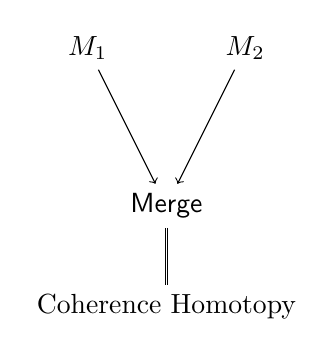
\begin{tikzpicture}[node distance=2cm, auto]
  \node (M1) {$M_1$};
  \node (M2) [right of=M1] {$M_2$};
  \node (Merge) [below of=M1, xshift=1cm] {$\mathsf{Merge}$};
  \draw[->] (M1) -- (Merge);
  \draw[->] (M2) -- (Merge);
  \draw[double] (Merge) -- +(0,-1) node[below] {Coherence Homotopy};
\end{tikzpicture}

\subsection{CLIO’s Recursive Inference Loop}

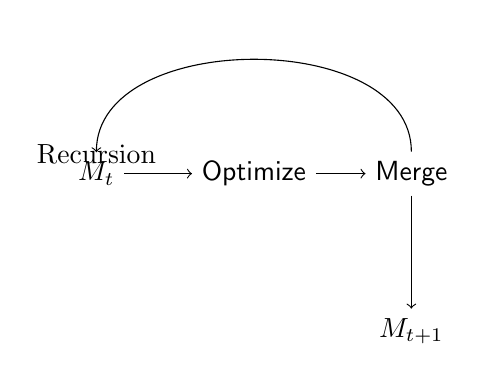
\begin{tikzpicture}[node distance=2cm, auto]
  \node (Mt) {$M_t$};
  \node (Opt) [right of=Mt] {$\mathsf{Optimize}$};
  \node (Merge) [right of=Opt] {$\mathsf{Merge}$};
  \node (Mt1) [below of=Merge] {$M_{t+1}$};
  \draw[->] (Mt) -- (Opt);
  \draw[->] (Opt) -- (Merge);
  \draw[->] (Merge) -- (Mt1);
  \draw[->, loop above] (Merge) to[out=90,in=90] (Mt) node[above] {Recursion};
\end{tikzpicture}

\subsection{Entropy Flow}

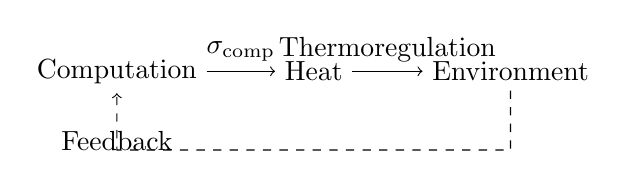
\begin{tikzpicture}[node distance=2.5cm, auto]
  \node (Comp) {Computation};
  \node (Heat) [right of=Comp] {Heat};
  \node (Env) [right of=Heat] {Environment};
  \draw[->] (Comp) -- (Heat) node[midway,above] {$\sigma_{\text{comp}}$};
  \draw[->] (Heat) -- (Env) node[midway,above] {Thermoregulation};
  \draw[->, dashed] (Env) -- +(0,-1) -- +(-5,-1) -- (Comp) node[midway,below] {Feedback};
\end{tikzpicture}

\bibliographystyle{plain}
\bibliography{entropy_as_infrastructure}
\end{document}
